\chapter{KELP MODEL}
\label{chap:kelp}

In order to properly model the spatial distribution of light around the kelp, it is first necessary to formulate a spatial description of the kelp.
Probability distributions are given for the size and orientation of the individual kelp fronds, which are inverted to determine the probability of a point in space being occupied by kelp.
Ultimately, the kelp density at any point in space is calculated, which informs the absorption coefficient of the effective kelp--water medium.


\section{Physical Setup}
The life of cultivated macroalgae generally begins in the laboratory, where microscopic kelp spores are inoculated onto a thread in a small laboratory pool.
This thread is wrapped around a larger rope as in Figure \ref{fig:rope_thread}, which is hung from buoys in the ocean.
The two primary configurations are vertical and horizontal or ``long'' lines.
In the case of vertical lines, the seaweed rope hangs straight down from a single buoy, and is either weighted or anchored.
In the case of long lines, the rope is strung from one buoy to another.
Long lines allow more light to reach the seaweed since it grows closer to the surface, but more vertical lines can be set up in a given area,
which may be advantageous for IMTA.

\begin{figure}[H]
  \centering
  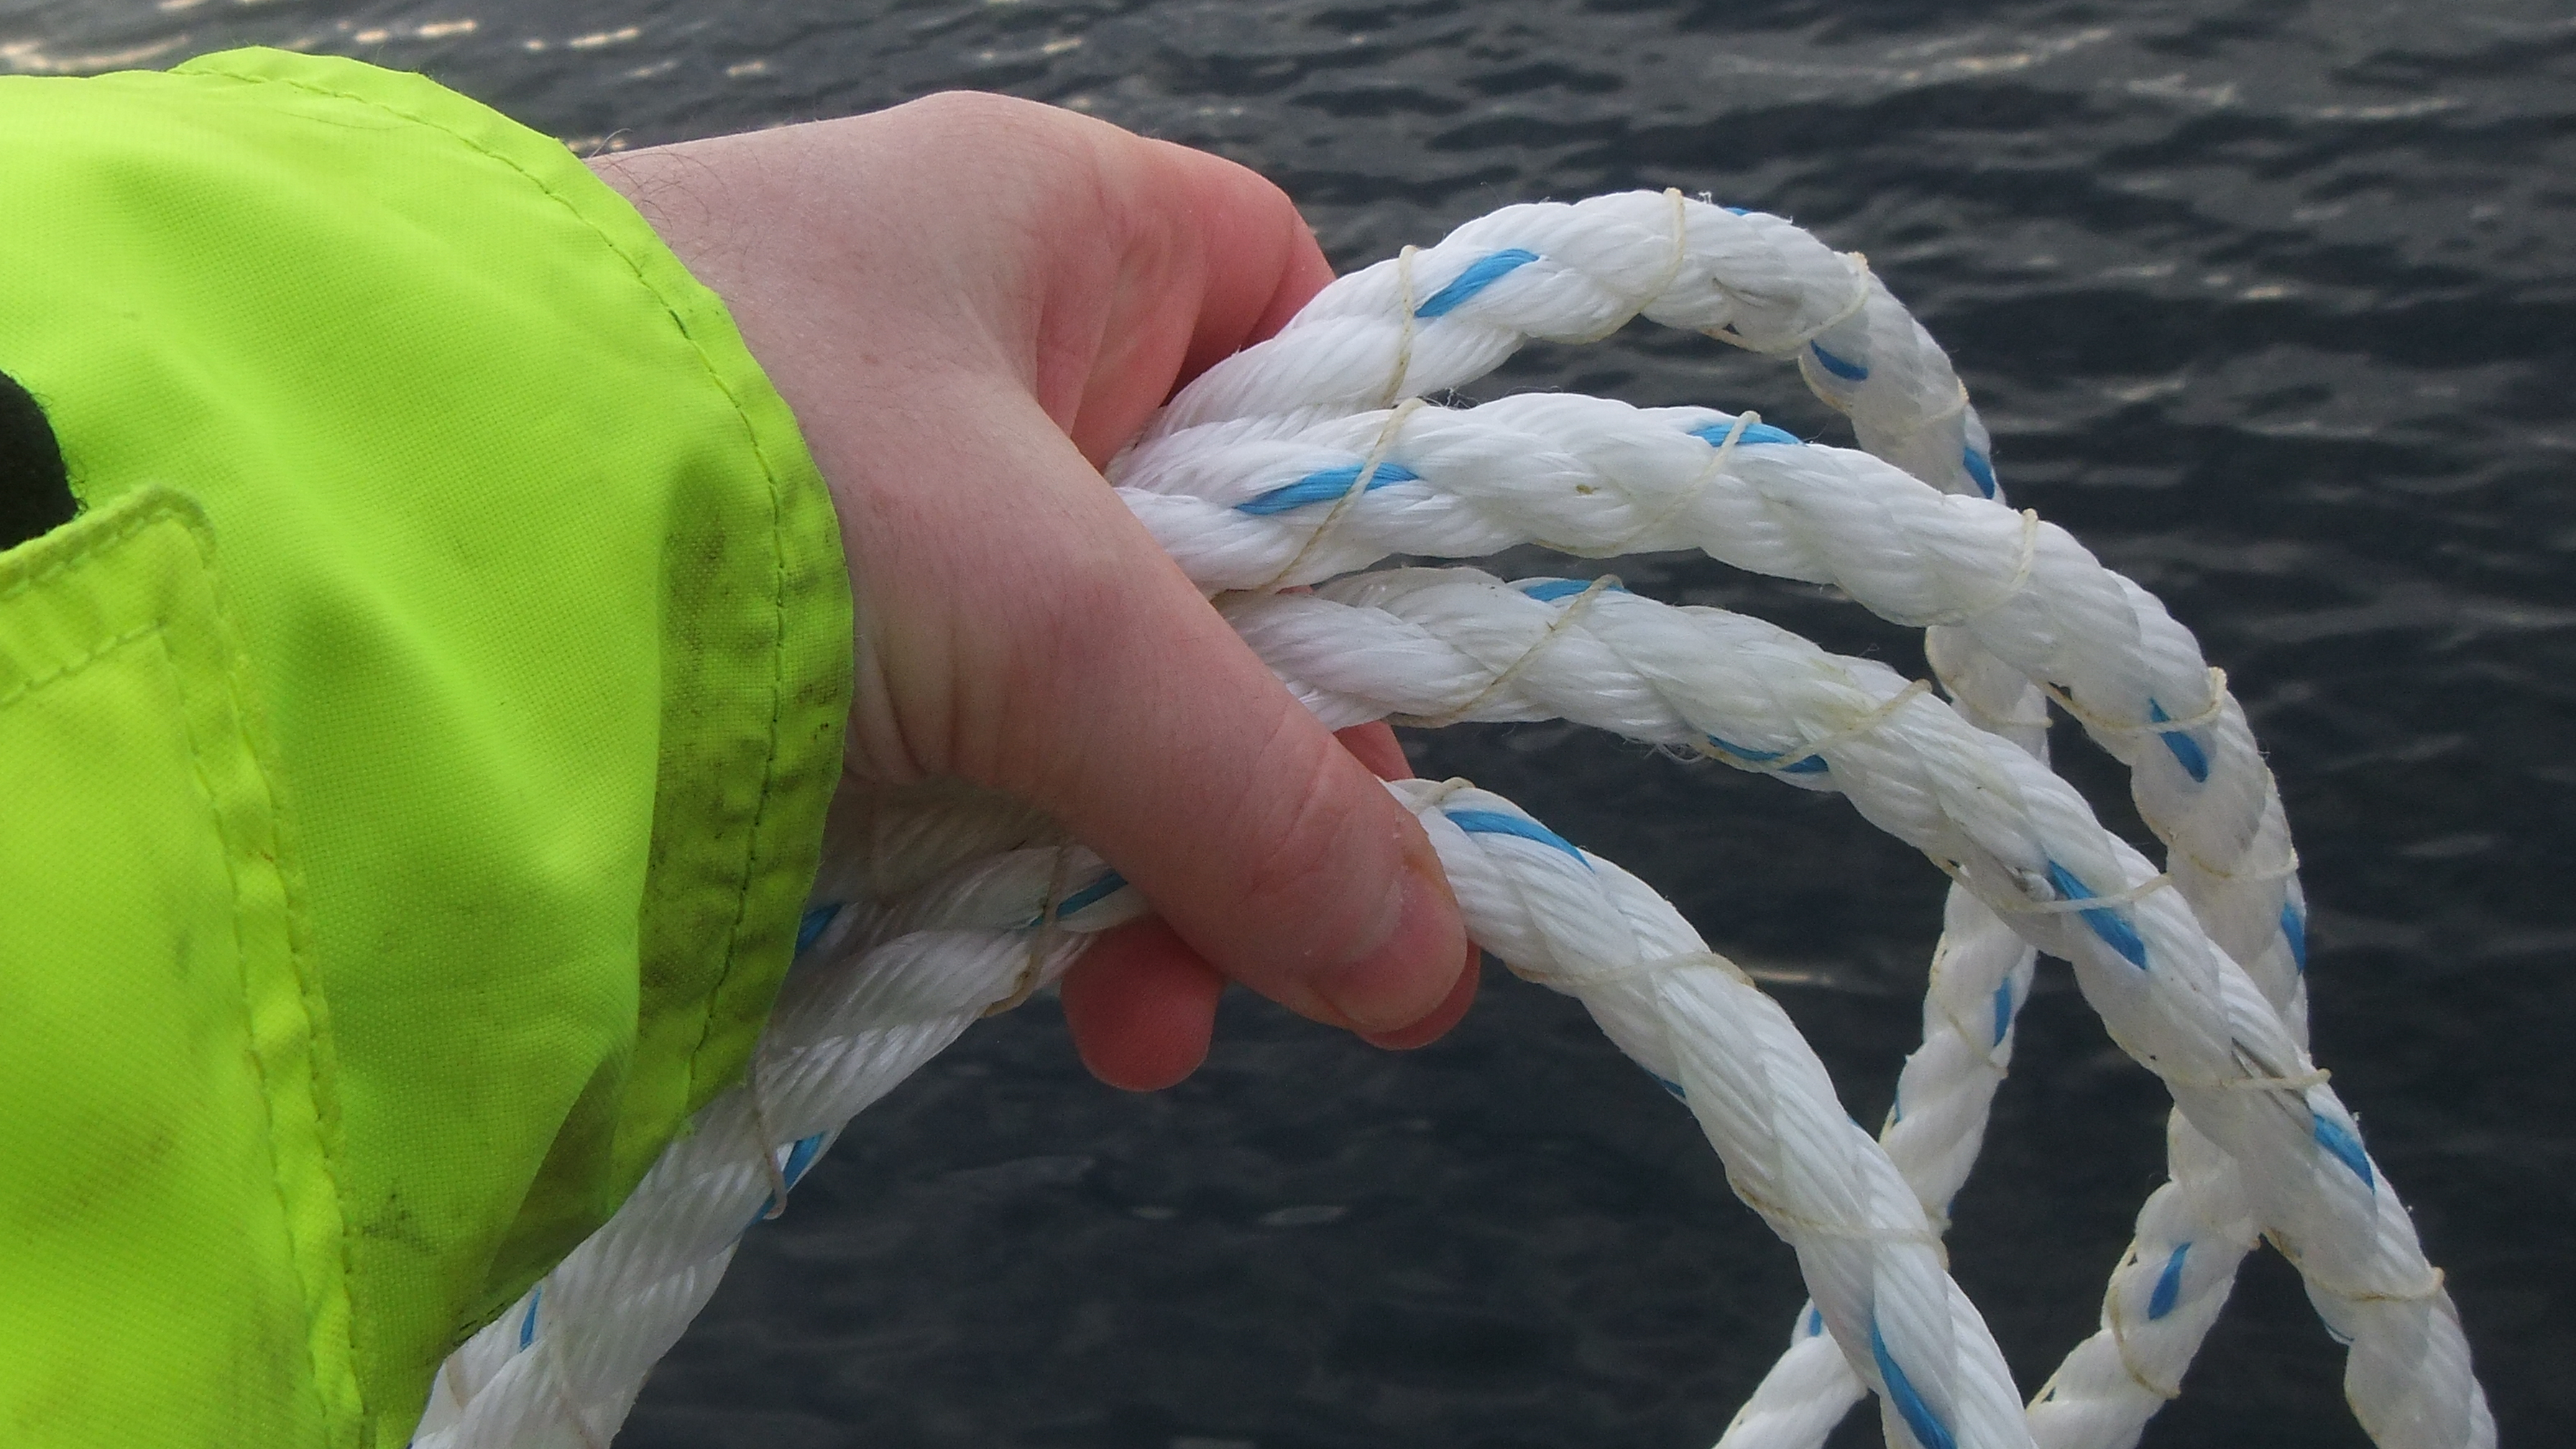
\includegraphics[width=0.65\textwidth]{kelp_photo/rope_thread}
  \caption{\textit{Saccharina latissima} inoculated onto a thread wrapped around a rope on which it is to be grown.}
  \label{fig:rope_thread}
\end{figure}

We consider only the case of a rigid vertical rope which does not sway in the current.
The mature \textit{Saccharina latissima} plant consists of a single frond (leaf), a stipe (stem) and a holdfast (root structure).
For the sake of this model, only the kelp frond is considered, and its base is attached directly to the rope.
The ``gentle undulation approximation'' is employed, whereby the fronds are modeled as perfectly horizontal.
While at any given time they may point up or down due to water current and gravity, we consider the horizontal
state to be an average configuration.
This simplification allows for the three--dimensionally distributed population of kelp fronds
to be considered a collection of independent populations in two--dimensional depth layers.
A computer rendering of this scenario is shown in Figure \ref{fig:kelp_array}.

\begin{figure}[H]
	\centering
	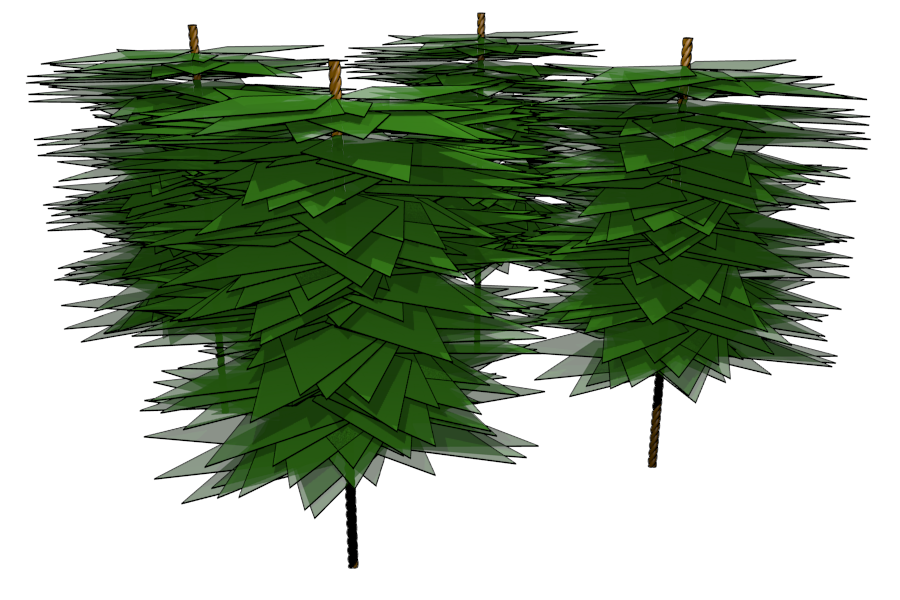
\includegraphics[width=3.5in]{kelp_array}
	\captionof{figure}{Rendering of four nearby vertical kelp ropes as represented in the spatial distribution model. Note the kite--shaped fronds and horizontal orientation.}
  \label{fig:kelp_array}
\end{figure}

\section{Coordinate System}
Consider the rectangular domain
\begin{align*}
  \xmin &\leq x \leq \xmax, \\
  \ymin &\leq y \leq \ymax, \\
  \zmin &\leq z \leq \zmax.
\end{align*}
For all three dimensional analysis, we use the absolute coordinate system defined in Figure \ref{fig:3dcoords}.
The vectors $\vec{x}=(x,y,z)$ and $\vec{\omega}=(\sin\phi\cos\theta, \sin\phi\sin\theta, \cos\phi)$ are also used throughout.
Also, the notation $\hat{x}$, $\hat{y}$, $\hat{z}$ is used for the Cartesian unit vectors.

In the following sections, it is necessary to convert between Cartesian and spherical coordinates, which we do using the relations
\begin{equation}
  \left\{
	\begin{split}
		x & = r\sin\phi\cos\theta, \\
		y & = r\sin\phi\sin\theta, \\
		z & = r\cos\phi. \\
	\end{split}
  \right.
	\label{eqn:coords}
\end{equation}
Therefore, for some function $f(x,y,z)$, we can write its derivative along a path in spherical coordinates in terms of Cartesian coordinates using the chain rule,
\begin{equation*}
	\frac{\partial f}{\partial r}
	=\frac{\partial f}{\partial x}\frac{\partial x}{\partial r}
	+ \frac{\partial f}{\partial y}\frac{\partial y}{\partial r}
	+ \frac{\partial f}{\partial z}\frac{\partial z}{\partial r}.
\end{equation*}
Then, calculating derivatives from \eqref{eqn:coords} yields
\begin{equation}
	\frac{\partial f}{\partial r}
	=\frac{\partial f}{\partial x}\sin\phi\cos\theta
	+ \frac{\partial f}{\partial y}\sin\phi\sin\theta
	+ \frac{\partial f}{\partial z}\cos\phi.
	\label{eqn:partials}
\end{equation}
\begin{figure}[H]
	\centering
	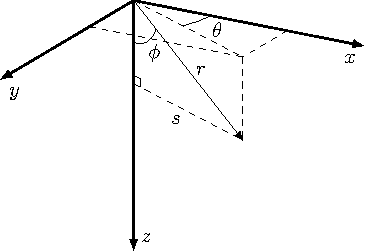
\includegraphics[width=3in]{3d_coords}
	\caption{Downward--facing right--handed coordinate system with radial distance $r$ from the origin, distance $s$ from the $z$ axis, zenith angle $\phi$ and azimuthal angle $\theta$.}
	\label{fig:3dcoords}
\end{figure}

\section{Population Distributions}
In order to construct a spatial distribution of kelp fronds, a simple kite--shaped geometry is introduced,
and frond lengths and azimuthal orientations are assumed to be distributed predictably.
Since it is assumed that fronds extend perfectly horizontally, no angular elevation distribution is required.

\subsection{Frond Shape}
\label{sec:shape}

\begin{figure}[h]
	\centering
  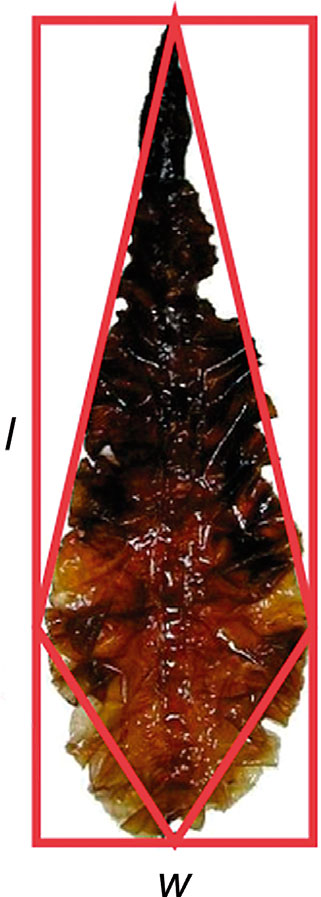
\includegraphics[width=1.2in]{kelp_photo/kite}
  %TODO: Cite this?
  \qquad
	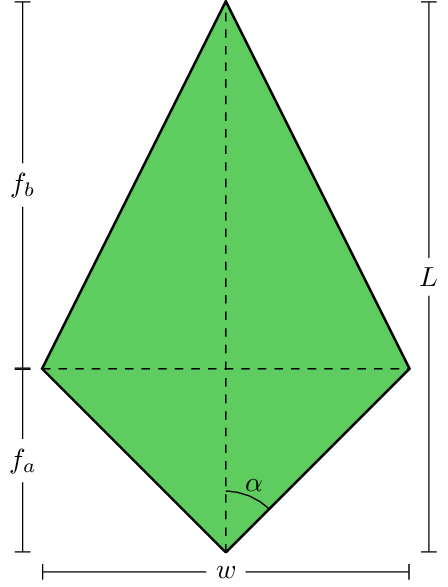
\includegraphics[width=2in]{frond}
	\captionof{figure}{Simplified kite--shaped frond. Reproduced with permission from \cite{broch_modelling_2013}.}
	\label{fig:frond}
\end{figure}

The frond is assumed to be kite--shaped with length $l$ from base to tip, and width $w$ from left to right.
In Figure \ref{fig:frond}, the base is shown at the bottom and the tip is shown at the top.
The proximal length is the shortest distance from the base to the diagonal connecting the left and right corners, and is notated as $f_a$.
Likewise, the distal length, notated $f_b$, is the shortest distance from that diagonal to the tip.
It is therefore clear that
 \begin{equation*}
	 f_a + f_b = l.
 \end{equation*}
When considering a whole population with varying sizes, it is more convenient to specify ratios than absolute lengths.
Define the ratios
\begin{align*}
	f_r &= \frac{l}{w}, \\
	f_s &= \frac{f_a}{f_b}.
\end{align*}
These ratios are assumed to be constant among the entire population, so that all fronds are geometrically similar.
Thus, the shape of the frond can be fully specified by $l$, $f_r$, and $f_s$;
it is possible to redefine $w$, $f_a$ and $f_b$ from the preceding formulas as
\begin{align*}
	w &= \frac{l}{f_r}, \\
	f_a &= \frac{lf_s}{1+f_s}, \\
	f_b &= \frac{l}{1+f_s}.
\end{align*}
The angle $\alpha$, half of the angle at the base corner, is also noteworthy.
From the above equations, it follows that
\begin{equation*}
	\alpha = \tan^{-1}\left(\frac{2f_rf_s}{1+f_s}\right).
\end{equation*}

It is useful to convert between frond length and surface area, which can be done via the relations
\begin{align}
  A &= \frac{lw}{2} = \frac{l^2}{2f_r},
  \label{eqn:area_from_length} \\
  l &= \sqrt{2Af_r}.
  \label{eqn:length_from_area}
\end{align}

\subsection{Length and Angle Distributions}
\label{sec:dist}
In any given depth layer, the distribution of frond lengths is assumed to be normal, with mean $\mu_l$ and standard deviation $\sigma_l$.
That is, it has the probability density function (PDF)
\begin{equation*}
  P_l(l) = \frac{1}{\sqrt{2\pi\sigma_l^2}}\exp\left(-\frac{(l-\mu_l)^2}{2\sigma_l^2}\right).
\end{equation*}

It is further assumed that frond orientation angle varies according to the von Mises distribution, which is the periodic analogue of the normal distribution, defined on $[-\pi,\pi]$ rather than $(-\infty,\infty)$.
The von Mises distribution has two parameters, $\mu$ and $\kappa$, which shift and sharpen its peak respectively, as shown in Figure \ref{fig:vonmises}.
$\kappa$ is analogous to $1/\sigma$ in the normal distribution.
In the absence of current, the frond angles are distributed uniformly, while as current velocity increases, they become increasingly likely to align parallel to the current, depending on the stiffness of the frond and stipe.
Assuming a linear relationship between the current velocity and the steepness of the angular distribution, define the \textit{frond alignment coefficient} $\eta$, with units of inverse velocity(\SI{}{\s\per\m}).
Then, use $\mu = \theta_w$ and $\kappa = \eta v_w$ as the von Mises distribution parameters.
Note that $\theta_w$ and $v_w$ vary over depth, while $\eta$ is assumed constant for the population.
Then, the PDF for the von Mises frond angle distribution is
\begin{equation*}
	P_{\theta_f}(\theta_f) = \frac{\exp\left(\eta v_w\cos(\theta_f-\theta_w)\right)}{2\pi I_0(\eta v_w)},
\end{equation*}
where $I_0(x)$ is the modified Bessel function of the first kind of order 0.
Notice that unlike the normal distribution, the von Mises distribution approaches a \textit{non--zero} uniform distribution as $\kappa$ approaches 0, so
\begin{equation*}
	\displaystyle \lim_{v_w \to 0}P_{\theta_f}(\theta_f) = \frac{1}{2\pi} \;\forall\, \theta_f \in [-\pi,\pi].
\end{equation*}

\begin{figure}[h]
	\centering
	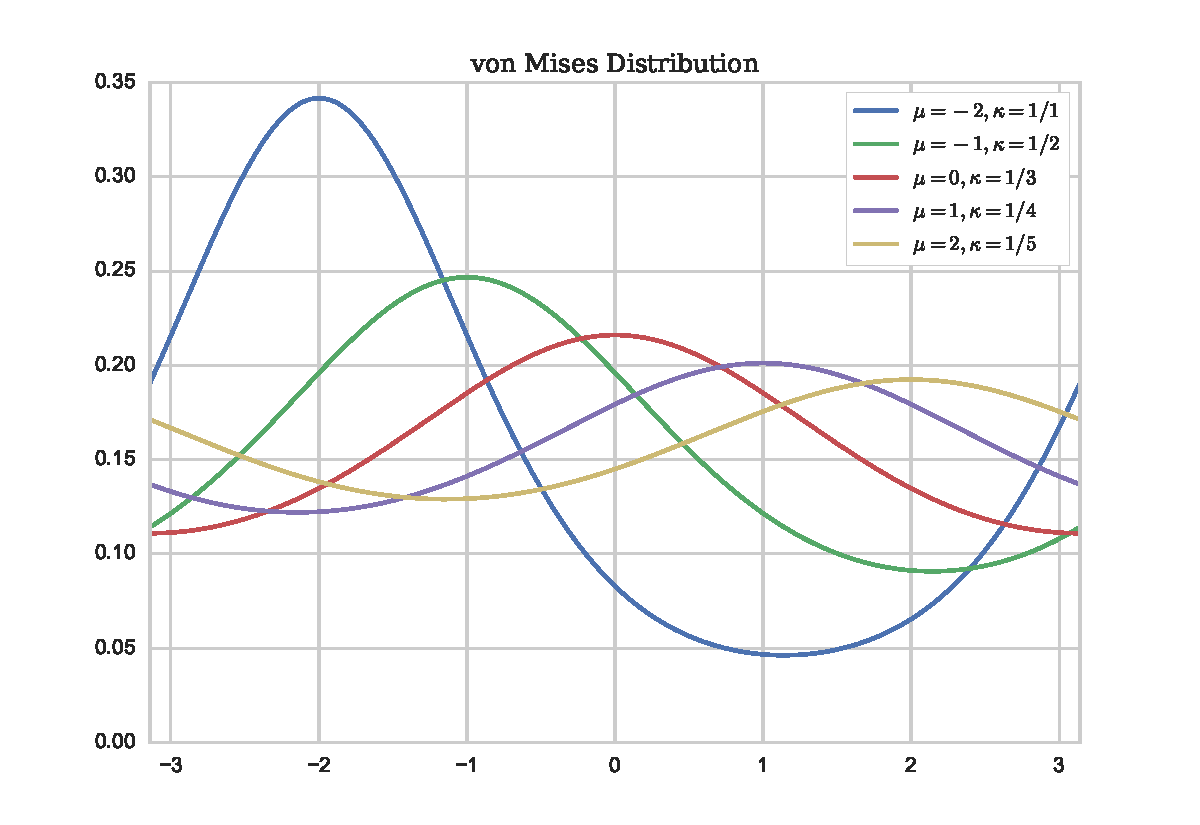
\includegraphics[width=6in]{vonmises}
	\captionof{figure}{von Mises distribution for a variety of parameters.}
	\label{fig:vonmises}
\end{figure}

\subsection{Joint Length--Orientation Distribution}
\label{sec:dist_2d}
The previous two distributions can reasonably be assumed to be independent of one another. That is, the angle of the frond does not depend on the length, or vice versa.
Therefore, the probability of a frond simultaneously having a given frond length and angle is the product of their individual probabilities.
Given independent events $A$ and $B$, the probability of their intersection is the product of their individual probabilities.
That is,
\begin{equation*}
	\label{eqn:ind_prob}
	P(A \cap B) = P(A)P(B).
\end{equation*}
Then the probability of frond length $l$ and frond angle $\theta_f$ coinciding is
\begin{equation}
  \label{eqn:p2d}
	P_{2D}(\theta_f,l) = P_{\theta_f}(\theta_f) \cdot P_l(l).
\end{equation}
A contour plot of this 2D distribution for a specific set of parameters is shown in Figure \ref{fig:dist_2d}, where probability is represented by color in the 2D plane.
Darker green represents higher probability, while lighter beige represents lower probability.
In Figure \ref{fig:kelp_sample}, 50 samples are drawn from this distribution and plotted.

It is important to note that if $P_{\theta_f}$ were dependent on $l$, the above definition of $P_{2D}$ would no longer be valid.
For example, it might be more realistic to say that larger fronds are less likely to bend towards the direction of the current.
In this case, \eqref{eqn:ind_prob} would no longer hold, and it would be necessary to use the more general Bayes' Theorem
\begin{equation*}
	P(A \cap B) = P(A)P(B|A) = P(B)P(B|A),
\end{equation*}
which is currently not taken into consideration in this model.

\begin{figure}[h]
	\centering
	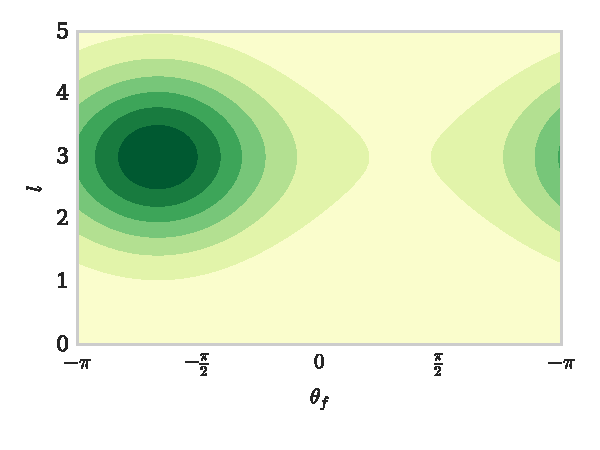
\includegraphics[width=4.5in]{prob_2d}
	\captionof{figure}{2D length--angle probability distribution with $\theta_w=7\pi/4$, $v_w=1$, $\mu_l=3$, $\sigma_l=1$.}
	\label{fig:dist_2d}
\end{figure}

\begin{figure}[h]
	\centering
	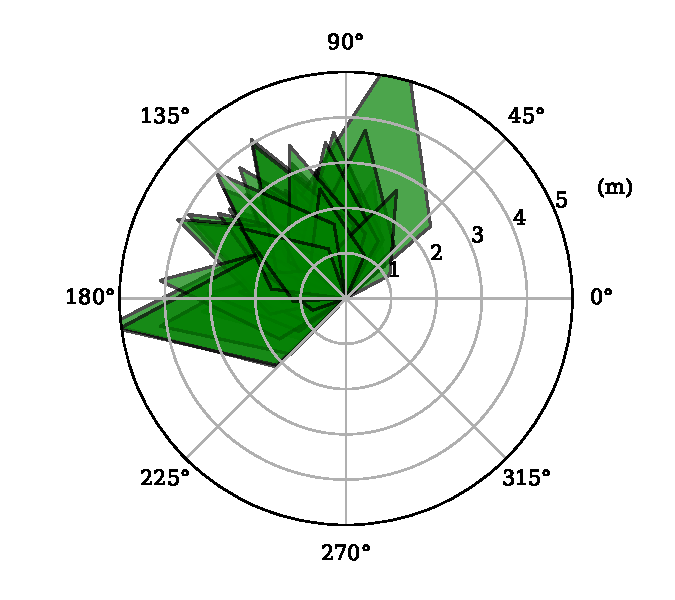
\includegraphics[width=4.5in]{kelp_sample}
	\captionof{figure}{A sample of 50 kelp fronds with shape parameters $f_s=0.5$ and $f_r=2$ whose lengths are picked from a normal distribution and whose angles are picked from a von Mises distribution.}
	\label{fig:kelp_sample}
\end{figure}

\section{Spatial Distribution}
In this section, the population length and angle distributions from the previous section are used to construct a spatial distribution of kelp.
This is made possible by the simple kite--shape fronds, and would be considerably more difficult with more general frond shapes.
\subsection{Rotated Coordinate System}
\label{sec:rot_coords}
To determine under what conditions a frond will occupy a given point, we begin by
describing the shape of the frond in Cartesian coordinates and then convert to polar coordinates.
Of primary interest are the edges connected to the frond tip.
For convenience, we will use a rotated polar coordinate system $(\theta',s)$ such that the line connecting the base to the tip points in the $+y$ direction ($\theta=\pi/2$), with the base at $(0,0)$.
Denote the Cartesian analogue of this coordinate system as $(x',y')$ which is related to $(\theta',s)$ by
\begin{align*}
	x' &= s\cos\theta' \\
	y' &= s\sin\theta' \\
	s &= \sqrt{x'^2+y'^2}, \\
	\theta' &= \atantwo(y, x).
\end{align*}

\subsection{Functional Description of Frond Edge}
With this coordinate system established, the outer two edges of the frond can be described in Cartesian coordinates as a piecewise linear function connecting the left corner: $(-w/2,f_a)$, the tip: $(0,l)$, and the right corner: $(w/2,f_a)$.
This function has the form
\begin{equation*}
	y'_f(x') = l-\sign(x')\frac{f_b}{w/2}x'.
\end{equation*}
Using the equations in Section \ref{sec:rot_coords}, this can be written in polar coordinates after some rearrangement as
\begin{equation*}
	s_f'(\theta';l) = \frac{l}{\sin\theta' + S(\theta')\frac{2f_b}{w}\cos\theta'},
\end{equation*}
where
\begin{equation*}
	S(\theta') = \sign(\cos\theta').
\end{equation*}
Then, using the relationships in Section \ref{sec:shape}, the above equation can be rewritten in terms of the frond ratios $f_s$ and $f_r$ as
\begin{equation}
	\label{eqn:rf_rel}
	s_f'(\theta';l) = \frac{l}{\sin\theta' + S(\theta')\frac{2f_r}{1+f_s}\cos\theta'}.
\end{equation}
For convenience, denote the denominator of \eqref{eqn:rf_rel} as $d_f'(\theta')$.
To generalize to a frond pointed at an angle $\theta_f$, we introduce the coordinate system $(\theta,s)$ such that
\begin{equation*}
	\theta = \theta' + \theta_f - \frac{\pi}{2}.
\end{equation*}
Then, for a frond pointed at the arbitrary angle $\theta_f$, the function for the outer edges can be written as
\begin{equation}
	\label{eqn:rf_abs}
	s_f(\theta;l) = s_f'\left(\theta - \theta_f + \frac{\pi}{2} \right).
\end{equation}
Similarly, define
\begin{equation}
	d_f(\theta) = d_f'\left(\theta - \theta_f + \frac{\pi}{2} \right).
\end{equation}

\subsection{Conditions for Occupancy}
We now formulate the conditions under which a kite shape frond occupies a point
in the sense that the point lies within its interior.
Combining these conditions with the size and orientation distributions from \ref{sec:dist}
allows a spatial distribution of the kelp fronds to be calculated.

Consider a fixed frond of length $l$ at an angle $\theta_f$. The point
$(\theta,s)$ is occupied by the frond if
\begin{align*}
	\left|\theta_f - \theta \right| < \alpha
  \mbox{ and }
	s < s_f(\theta).
\end{align*}
Equivalently, the opposite perspective can be taken.
Letting the point $(\theta,s)$ be fixed, a frond occupies the point if
\begin{align}
	\theta - \alpha < \theta_f < \theta + \alpha,
	\label{eqn:rs_th} \\
	l > l_{\min}(\theta,s),
	\label{eqn:rs_l}
\end{align}
where
\begin{equation}
	l_{\min}(\theta,s) = s \cdot \frac{l}{s_f(\theta;l)} = s \cdot d_f(\theta).
  \label{eqn:l_min}
\end{equation}
Then, considering the point to be fixed, \eqref{eqn:rs_th} and \eqref{eqn:rs_l} define the spacial region $R_s(\theta,s)$ called the ``occupancy region for $(\theta,s)$'' with the property that if the tip of a frond lies within this region (i.e., $(\theta_f,l) \in R_s(\theta,s)$), then it occupies the point.
$R_s(3\pi/4,1.5)$ is shown in blue in Figure \ref{fig:shade_area} and the smallest possible occupying fronds for several values of $\theta_f$ are shown in various colors.
Any frond longer than these at the same angle will also occupy the point.

\begin{figure}[h]
	\centering
	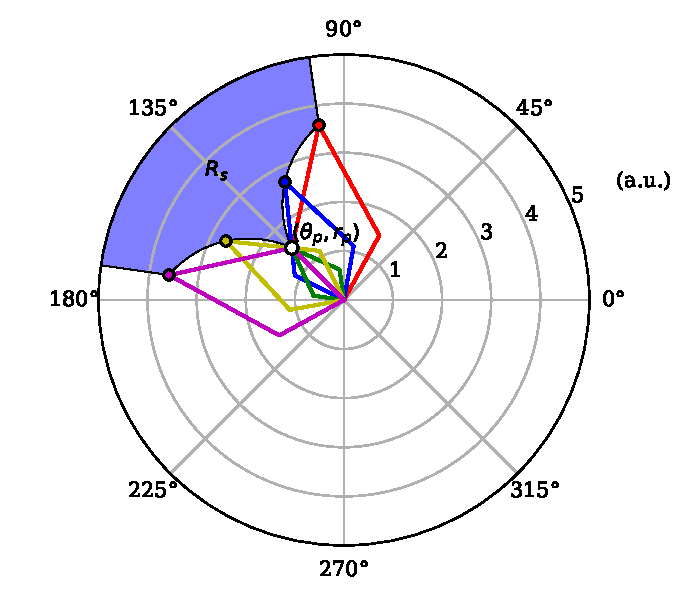
\includegraphics[width=4.5in]{shade_area}
	\captionof{figure}{Outlines of minimum--length fronds for a variety of angles to occupy the point $(\theta,s)=(3\pi/4,3/2)$.}
	\label{fig:shade_area}
\end{figure}

\subsection{Probability of Occupancy}
We are interested in the probability that, given a fixed point $(\theta,s)$, values of $l$ and $\theta_f$ chosen from the distributions described in Section \ref{sec:dist} will fall in the occupancy region.
This is found by integrating $P_{2D}(\theta_f, l)$ from \eqref{eqn:p2d} over $R_s(\theta,s)$, the occupancy region for the point of interest.

\begin{figure}[h]
	\centering
	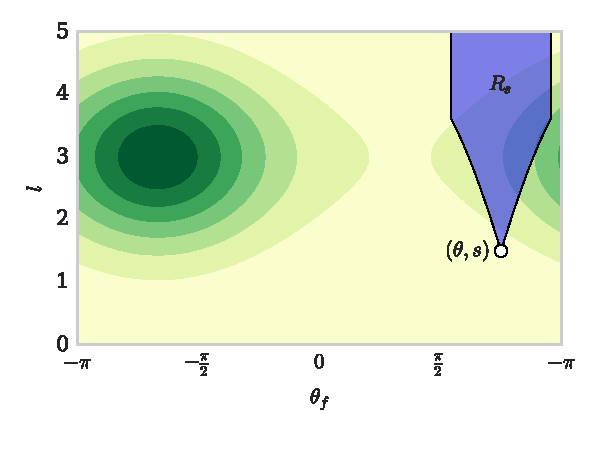
\includegraphics[width=4.5in]{cart_shade}
	\captionof{figure}{Contour plot of $P_{2D}(\theta_f,l)$ overlayed with the
    region in the $\theta_f$\nobreak--\nobreak$l$ plane which results in a frond occupying the point $(\theta,s)=(3\pi/4,3/2)$.}
	\label{fig:cart_shade}
\end{figure}

Integrating $P_{2D}(\theta_f,l)$ over $R_s(\theta,s)$ as depicted in Figure \ref{fig:cart_shade} yields the proportion of the population in the depth layer occupying the point $(\theta,s)$,
\begin{align}
		\tilde{P}_k(\theta,s,z)	&= \iint_{R_s(\theta,s)}
								P_{2D}(\theta_f,l)
								\,dl\,d\theta_f \nonumber \\
							&= \int_{\theta-\alpha}^{\theta+\alpha}
								\int_{l_{\min}(\theta_f)}^\infty
								P_{2D}(\theta_f,l)
								\,dl\,d\theta_f.
                \label{eqn:integrate_p2d}
\end{align}

Assuming that the depth layer has thickness $dz$ and contains $n_f$ fronds of thickness $f_t$,
the proportion of the vertical length of the discrete depth layer occupied by kelp at any position $(x,y,z)$ is given by
\begin{equation}
  P_k(x, y) = \frac{n_ff_t}{dz}\tilde{P}_k(x, y).
  \label{eqn:kelp_pk}
\end{equation}
In the continuum limit as the number of discrete depth depth layers approaches infinity, $P_k(x,y,z)$ can be interpreted as the probability of the point $(x,y,z)$ being occupied by kelp.
In a three dimensional context, the number of fronds is more likely to be specified by a number density $\rho_f=n_f/dz$ over the vertical length of the rope with units \SI{}{\per\m}, in which case
\begin{equation}
  P_k(x, y, z) = f_t \rho_f(z) \tilde{P}_k(x, y, z).
\end{equation}
Then, since the point $\vec{x}$ has a probability $P_k(\vec{x})$ of being occupied by kelp and a probability $(1-P_k(\vec{x}))$ of being occupied by the surrounding aquatic medium,
the effective absorption coefficient can be calculated as
\begin{equation*}
  \label{eqn:abs_field}
  a(\vec{x}) = P_k(\vec{x})a_k + (1-P_k(\vec{x}))a_w,
\end{equation*}
where $a_k$ is the absorption coefficient of the kelp alone, and $a_w$ is the absorption coefficient of the water and its dissolved and suspended contents.

\begin{figure}[h]
	\centering
	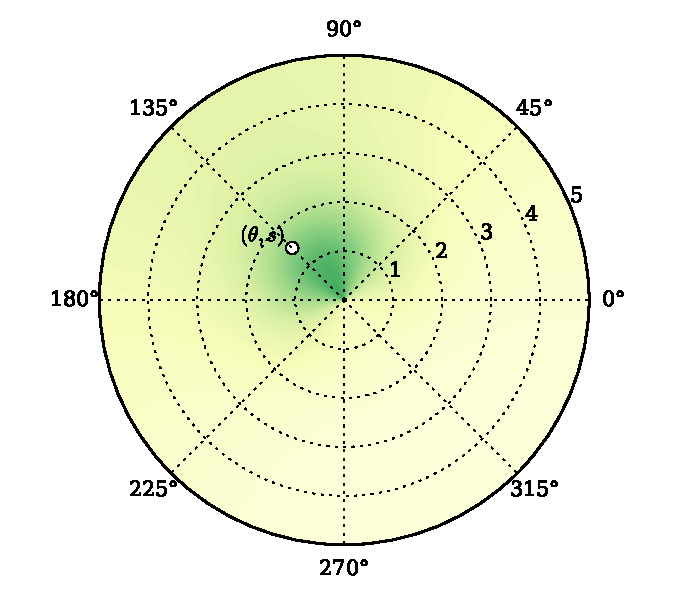
\includegraphics[width=4.5in]{prob_shade}
	\captionof{figure}{Contour plot of the probability of frond occupation sampled at 121 points using $\theta_f=2\pi/3,\eta v_w=1$.}
	\label{fig:prob_shade}
\end{figure}

\section{Discontinuity at the Rope}
While the above model of the kelp distribution is straightforward to evaluate, it does have a significant numerical difficulty in its application.
Since the length and orientations are both continuous in the polar coordinates $s>0$ and $\theta$, the resulting kelp density and effective absorption coefficient are as well.
However, they are not necessarily continuous in Cartesian coordinates.
In the case of no water current, $v_w=0$, the flat von Mises distribution produces a continuous solution at the origin.
In the more general case, though, there is a high kelp density on one side of the origin in the direction of the current, and a low kelp density immediately on the other side.
Since the rope is assumed to be infinitely thin and have a fixed position, the sharp corners of the kelp fronds emanate from exactly the same point.
Hence, there is in general a discontinuity in the kelp distribution at the origin, and therefore its derivatives are unbounded on the domain.

This is not appealing numerically since the algorithms used in this thesis to solve the differential equation describing the light field are based on interpolation on a discrete Cartesian grid.
According to Taylor's theorem, the error incurred by performing such interpolation is bounded by a constant multiple of the appropriate maximum derivative of the interpolated function over the domain.
If the derivatives of the absorption coefficient are unbounded, then so too is the discretization error in the final solution.
That is, the solution is not guaranteed to converge.

Luckily, there is a straightforward solution, which is to post--process the spatial kelp distribution with a Gaussian blur in the $x$ and $y$ dimensions.
This is achieved via convolution of the solution with a 2D Gaussian kernel centered at the origin.
Any blur whatsoever is sufficient to bound the derivatives, and the larger the blur radius, the smaller they become.
Obviously, as the blur radius is increased, the kelp distribution tends toward a constant and no longer captures any information about the $xy$ distribution of the kelp.
Therefore, a small blur radius should be used.

\subsection{One dimensional Gaussian Blur}
As a one dimensional analogy, consider the Heaviside step function,
\begin{equation*}
  H(x) = \begin{cases}
    0, & x < 0, \\
    1, & x > 0.
  \end{cases}
\end{equation*}
Clearly, the function is infinitely steep at the origin.
Consider the normalized Gaussian kernel centered at the origin with radius $\sigma_b$, given by
\begin{equation}
  k(x;\sigma_b) = \frac{1}{\sqrt{2\pi\sigma_b^2}} \exp\left({-\frac{x^2}{2\sigma_b^2}}\right).
\end{equation}
A blur is applied by convolving the function with the kernel according to the formula
\begin{align*}
  \tilde{H}(x) &= (k*H)(x) = \int_{-\infty}^{\infty}H(\tau)k(x-\tau;\sigma_b)\, d\tau \\
  &= \int_{0}^{\infty}k(x-\tau;\sigma_b)\, d\tau.
\end{align*}
The substitution $u=\tau=x,\, du=d\tau$ yields
\begin{equation*}
  \tilde{H}(x) = \int_{-x}^\infty k(u;\sigma_b)\, du.
\end{equation*}
Note that since the kernel is normalized, the integral from 0 to infinity is $1/2$.
Further, since the kernel is even, the integral over $[-x, 0]$ is equal to the integral over $[0, x]$.
Hence,
\begin{equation*}
  \tilde{H}(x) = \frac{1}{2} + \int_{0}^x k(u;\sigma_b)\, du.
\end{equation*}
Then, by the fundamental theorem of calculus, the derivative of the convolved function is simply $k(x;\sigma_b)$, whose maximum value is $k(0;\sigma_b) = 1/\sqrt{2\pi\sigma_b^2}$.
Then, since the derivative is a linear operator, this result can be generalized to the following statement:
Applying a Gaussian blur of radius $\sigma_b$ to a function with a maximum discontinuity of size $J$ produces a function whose first derivative is bounded by
\begin{equation*}
  \frac{1}{\sqrt{2\pi}}\frac{J}{\sigma_b}.
\end{equation*}
The same logic applies to directional derivatives of multidimensional scalar functions.

\subsection{Multidimensional Gaussian Blur}
\label{sec:gaussian_blur}
In light of the above arguments, the derivatives of the absorption coefficient are bounded by applying a Gaussian blur to $P_k$ before the calculation of $a(\vec{x})$.
This is done by convolving slices of $P_k$ in the $xy$--plane with the two--dimensional normalized Gaussian kernel
\begin{equation}
  \label{eqn:gaussian_kernel}
  K(x, y; \sigma_b) = \frac{1}{\sqrt{2\pi\sigma_b^2}} \exp\left(\frac{x^2 + y^2}{2\sigma_b^2}\right).
\end{equation}
Hence, the blurred solution is 
\begin{equation}
  \label{eqn:gaussian_blur}
  P_k^b(x, y, z) = \int_{-\infty}^\infty \int_{-\infty}^\infty K(x', y', z; \sigma_b) P_k(x-x', y-y', z)\, dx'\, dy'.
\end{equation}
A physical interpretation of this Gaussian blurring is that $P_k^b$ is the time--averaged kelp distribution, assuming that the rope is allowed to move horizontally, and $k(x, y; \sigma)$ is the PDF of the rope's location distribution.
This interpretation is a bit incongruous with the rest of the model since there is no other explicit mention of time--averaging; while the frond length and position distributions can be thought of as continuous approximations to the population distribution at a single point in time, this idea does not apply to the rope's position, since there is only one rope.

\subsection{Absorption Coefficient Plots}
A variety of numerically calculated absorption coefficient fields are shown here in order to demonstrate some key features of the kelp distribution.
In each figure, the absorption coefficient is plotted on the color axis, while the norm of its gradient is shown with contours, with brighter contour lines indicating regions of large derivatives.
As mentioned above, large derivatives generate large discretization error, and are therefore undesirable.
Of course, the distributions must be sufficiently well--defined to capture the characteristics of the kelp.
Note that all of the kelp distributions are periodic in order to easily represent multiple vertical lines grown in close proximity.

Figure \ref{fig:abs_coefs_combined}(a) shows a sharp kelp distribution with an unrealistically high current velocity, with all fronds identically equal in length, and with no blurring applied.
Note the kite--shaped distribution, as expected.
Also note the regions of high derivatives near the origin and inner edges.
This sharp distribution requires excessively large numerical grids to approximate well, and is therefore undesirable.

In Figure \ref{fig:abs_coefs_combined}(b), the current velocity has been reduced, and a nonzero standard deviation has been given to the frond distribution.
With a variety of frond lengths, the edges are no longer as clearly defined, although the general character of the distribution is sensible --- the kelp is most dense near the rope in the direction of the current.
However, note that there remains a small neighborhood of sharp derivatives encompassing the origin.
Such a distribution may still cause numerical difficulties for the numerical algorithm.

Figure \ref{fig:abs_coefs_combined}(c) is similar to Figure \ref{fig:abs_coefs_combined}(b), except it has been post--processed with a moderate Gaussian blur of radius \SI{40}{cm}, not so large that it significantly distorts the shape of the distribution, but sufficient to remove the discontinuity in the origin.
Such a kelp distribution is ideal, as it balances accuracy with ease of numerical approximation.

In Figure \ref{fig:abs_coefs_combined}(d), too large of a blur has been applied; the character of the Gaussian kernel has overwhelmed that of the kelp distribution.
While this may still provide a better spatial description of the kelp than a fully horizontally uniform distribution, and unnecessary amount of information has been sacrificed for marginal gains in smoothness over Figure \ref{fig:abs_coefs_combined}(c).
Such a large blur is unlikely to reduce the discretization error since other factors discussed later contribute to discretization error as well.
\begin{figure}[H]
  \centering
  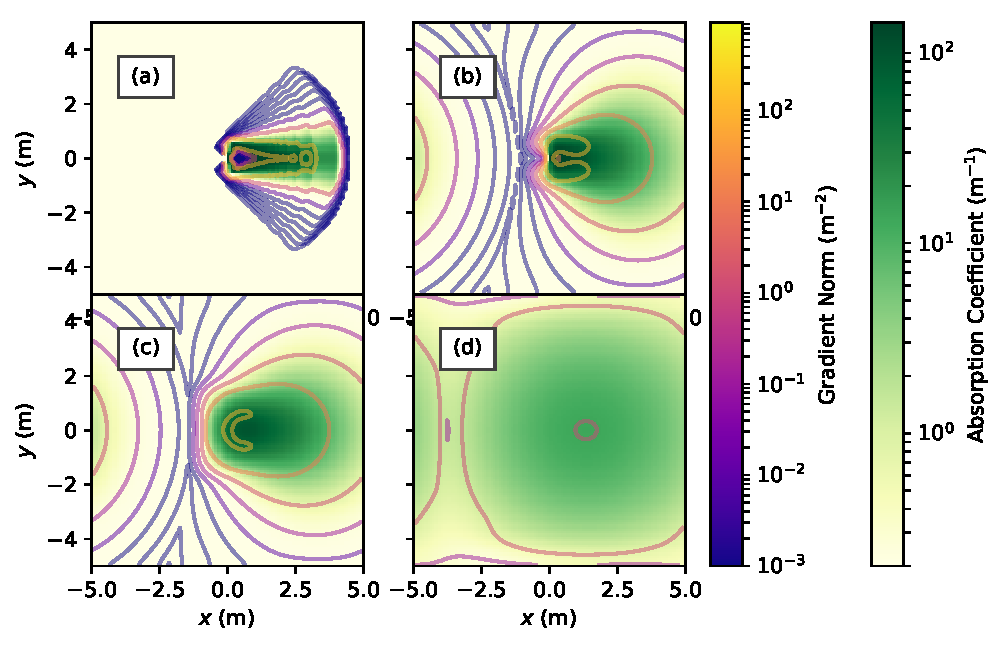
\includegraphics[width=6in]{abs_coefs_combined}
  \caption{$z$--slices of several absorption coefficient distributions from kelp distributions with varying parameters. The norm of the gradient is depicted with contours. (a) $\eta v_w=90$, $\sigma_l=\sigma_b=0$. Unrealistically sharp distribution shows kite--shaped character. (b) $\eta v_w=10$, $\sigma_b=0$, $\sigma_l=\SI{1}{\m}$. More realistic kelp distribution, but still has large derivatives near the origin. (c) $\eta v_w=10$, $\sigma_b=\SI{0.4}{\m}$, $\sigma_l=\SI{1}{\m}$. Moderate Gaussian blur slightly reduces derivatives near the origin. (d) $\eta v_w=10$, $\sigma_b=\SI{2}{\m}$, $\sigma_l=\SI{1}{\m}$. Over--blurred distribution; should be avoided.}
  \label{fig:abs_coefs_combined}
\end{figure}
